\section{Sprachaufbau der UML 2.0}

UML ist kein verbindlicher ISO-Standard, erfährt aber trotzdem eine hohe Akzeptanz durch die Industrie.\\

Die Spezifikation von UML (\cite{UML17}) durch die \textbf{OMG} (\textit{Object Management Group}\footnote{
    \url{https://omg.org}, abgerufen 29.04.2024
}) umfasst vier Teile:

\begin{itemize}
    \item \textbf{UML 2.0 Superstructure}: Definiert 6 verschiedene \textit{Strukturdiagramme}, 3 \textit{Verhaltensdiagramme}, 4 \textit{Interaktionsdiagramme}\footnote{
    diese Spezifikation ist Grundlage für die Arbeit der Toolhersteller
    }
    \item \textbf{UML 2.0 Infrastructure}: Definiert grundlegende Modellierungskonzepte als Basis für die Entwicklung von UML 2.0
    \item \textbf{UML 2.0 Object Constraint Language}\footnote{
    \textit{OCL}, \url{https://www.omg.org/spec/OCL/}, abgerufen 29.04.2024
    }: Definiert eine formale Sprache zur Formulierung von \textit{Einschränkungen} (Vor-/nachbedingungen für Operationen, Wertebereiche von Datentypen, Definition von Modellierungskonzepten im UML Metamodell, \ldots))
    \item \textbf{UML 2.0 Diagram Interchange} (\textit{XMI}\footnote{
    \textit{XML Metadata Interchange}: \url{https://www.omg.org/spec/XMI}, abgerufen 30.04.2024
    }): Definiert ein Austauschformat auf Basis von XML, bspw. für Import-/Export von MOdellen in unterschiedlichen Tools
\end{itemize}


\noindent
Da der Kurs sich hauptsächlich mit der \textbf{Superstructure} beschäftigt, müssen zunächst die folgenden Begriffe geklärt werden:

\begin{itemize}
    \item \textbf{Modell}
    \item \textbf{Modellelement}
    \item \textbf{Modellierungskonzept}
    \item \textbf{Metamodell}
    \item \textbf{Diagramm}
\end{itemize}

\subsection*{Modell}
Abstraktion eines Gegenstandes oder Prozesses (s.a. Abschnitt~\ref{sec:modelle-in-analyse-und-entwurf}).\\
\textbf{Modelle} haben die Aufgabe, den Bezug zum Original (Programm, Softwaresystem) herzustellen, sowie zu der \textit{Anwendungsumgebung}.\\

\noindent
Diese \textit{Doppelfunktion} wird gut sichtbar in der \textbf{objektorientierten Modellierung}: Hier tragen konzeptionelle Objekte des Modells \textbf{Attribute} und \textbf{Operationen}, die die \textbf{Eigenschaften} und das \textbf{Verhalten} der \textbf{Bezugsobjekte} der Anwendungsumgebung wiedergeben\footnote{
    natürlich enstprechen die Ausprägungen nur dem Zweck der Objekte, nicht dem vollständigen Gegenstand / Prozess.
}.

\noindent
Ein UML Modell enthält alle \textbf{Modellelemente}, die zur Beschreibung eines Softwaresystems benötigt werden.\\
Die resultierende \textit{Systembeschreibung} beinhaltet sowohl Struktur als auch Verhalten, falls durch den Zweck bedingt.

\subsection*{Modellelement}
Ein \textbf{Modellelement} wird als Element in einem UML Modell von einem Benutzer erstellt, und wird durch die \textbf{UML Modellierungskonzepte} beschrieben.

\subsection*{Modellierungskonzepte}
Die Beschreibung der \textbf{Modellelemente} erfolgt durch die \textbf{Modellierungskonzepte}, die eine Metaklasse im Metamodell der UML darstellt.\\
Ein \textbf{Modellelement} ist eine \textit{Instanz} eines bestimmtem UML Modellierungskonzepts\footnote{
Modellierungskonzepte werden im UML Metamodell beschrieben.
}.
Bspw. ist \code{class} ein bekanntes Modellierungskonzept, aus dem bspw. ein Modellelement \code{Person} erzeugt werden kann, das in einem Klassendiagramm eines Softwaresystems verwendet wird.

\subsection*{Diagramm}
Ein \textbf{Diagramm} ist eine grafische Darstellung von Daten oder Informationen.\\
\textbf{Modellelemente} eines UML Models können auf verschiedenen Diagrammen platziert werden.\\
Diagramme können \textit{Struktur} oder \textit{Verhalten} visualisieren, weshalb Modellierungskonzepte der UML bestimmte grafische Notationen besitzen\footnote{
bspw. wird \code{class} als Rechteck dargestellt, eine Instanz davon im Klassendiagramm dann als Rechteck, das den Namen der Instanz trägt
}.

\subsection*{Metamodell}
Das UML \textbf{Metamodell} wird auf Basis des Metamodells der \textit{MOF}\footnote{
\textit{Meta Object Facility}, \url{https://www.omg.org/mof/}, abgerufen 29.04.2024
} definiert.\\
In der MOF werden grundlegende Konzepte definiert, die wiederum in der UML für die Definition der Modellierungskonzepte benötigt werden\footnote{
``[\ldots] ein kleiner Begriffsraum [wird] genutzt, um einen größeren zu erklären`` (\cite[5]{Buh09})
} (s. Abbildung~\ref{fig:metamodel}).

\begin{enumerate}
    \item Die \textbf{Metaebene} der MOF wird mit M3 bezeichnet.
    \item Das Metamodell der UML befindet sich auf Ebene M2.
    \item Die in der Praxis verwendeten Modellelemente bilden die dritte Ebene (M1) - Modellelemente werden aus Modellierungskonzepten instanziiert\footnote{
    die Kurseinheit beschäftigt sich mit den Modellierungskonzepten (Schicht M2) und den daraus entwickelten Modellen (Schicht M1)
    }.
\end{enumerate}

\noindent
Das Metamodell der UML sowie deren Verwendung zur Erstellung von Diagrammen wird in der Teil Superstructure der OMG Spezifikationen dokumentiert.\\
Die Erklärung der Konzepte basiert auf einer abstrakten Syntax, zu deren Beschreibung wiederum Klassendiagramme genutzt werden.
Regeln zur syntaktischen Korrektheit werden mittels der \textbf{OCL} beschrieben.
Die Bedeutung der Modellierungskonzepte wird textlich beschrieben.\\
Darüber hinaus werden die in der UML Superstructure erläuterten Modellierungskonzepte in Paketen zusammengefasst.


\begin{figure}
    \centering
    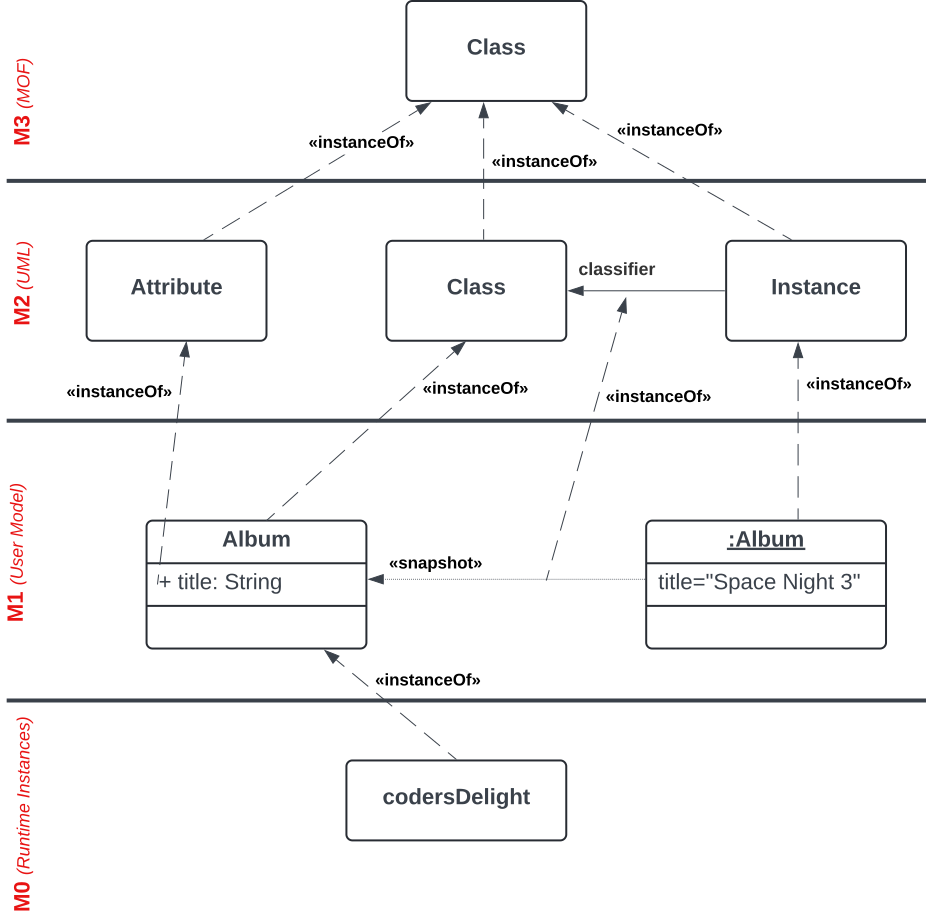
\includegraphics[scale=0.4]{part three/Einführung/img/metamodel}
    \caption{Beispiel für die verschiedenen Schichten der Metamodell Hierarchie. (Quelle: in Anlehnung an S. 20, Figure 7.8, \url{https://www.omg.org/spec/UML/2.4.1/Infrastructure/PDF}, abgerufen 01.05.2024}
    \label{fig:metamodel}
\end{figure}
